\subsection{DIRECT}
DIviding RECTangles (DIRECT) is a partitioning algorithm that recursively subdivides the feasible region into smaller hyperrectangles. The algorithm is as follows:
\begin{enumerate}
    \item Divide the feasible region into smaller hyperrectangles.
    \item Evaluate the function at the center of each hyperrectangle. The division is performed so that the region with the best function value is given the largest space.
    \item a set of potentially optimal hyperrectangles is identified and further divided.
\end{enumerate}
The stopping condition is either based on the maximum number of iterations / function evaluations or on the improvemnt of the function value. This means that the specific tolerance is dependent on the problem being solved. For example in the case of the De Jong's function \ref{fig:dejong-tolerance} we can see that different tollerance levels lead to different results.
\begin{figure}[H]
    \begin{subfigure}{0.5\textwidth}
        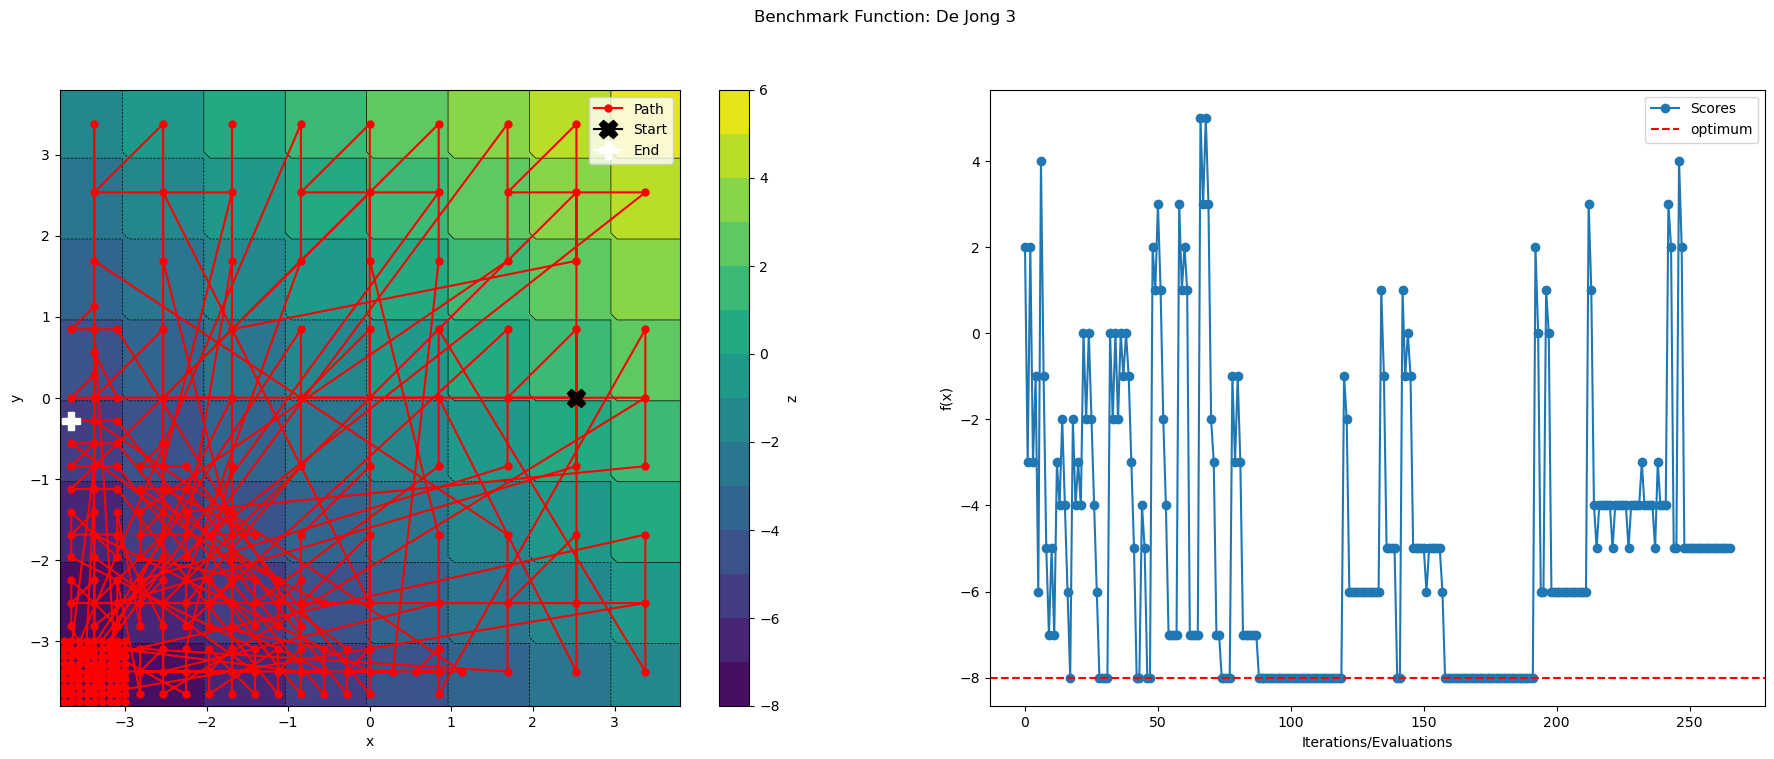
\includegraphics[width=\textwidth]{lab2/imgs/di_dejong_eps_01.png}
        \caption{$\epsilon =0.1$}
    \end{subfigure}
    \begin{subfigure}{0.5\textwidth}
        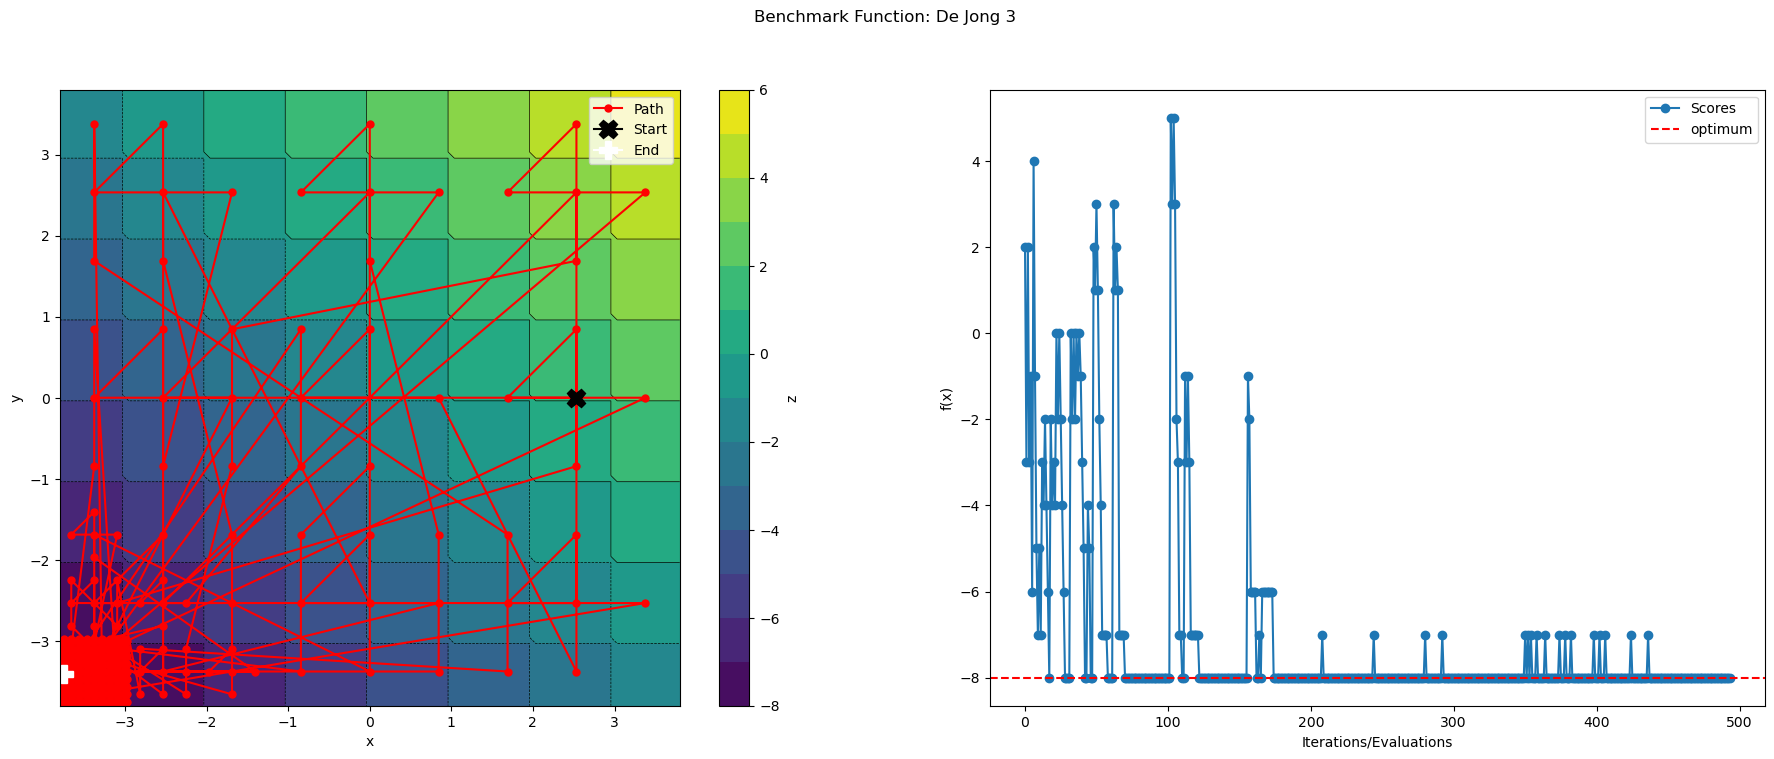
\includegraphics[width=\textwidth]{lab2/imgs/di_dejong_eps_001.png}
        \caption{$\epsilon =0.001$}
    \end{subfigure}
    \caption{DIRECT on De Jong's function with different tolerances}
    \label{fig:dejong-tolerance}
\end{figure}
For other functions, such as the Ackley function, the tolerance level does not have an impact on the results, probably bacause the function has a more clear basin of attraction towards the global minimum.
\begin{figure}[H]
    \begin{subfigure}{0.5\textwidth}
        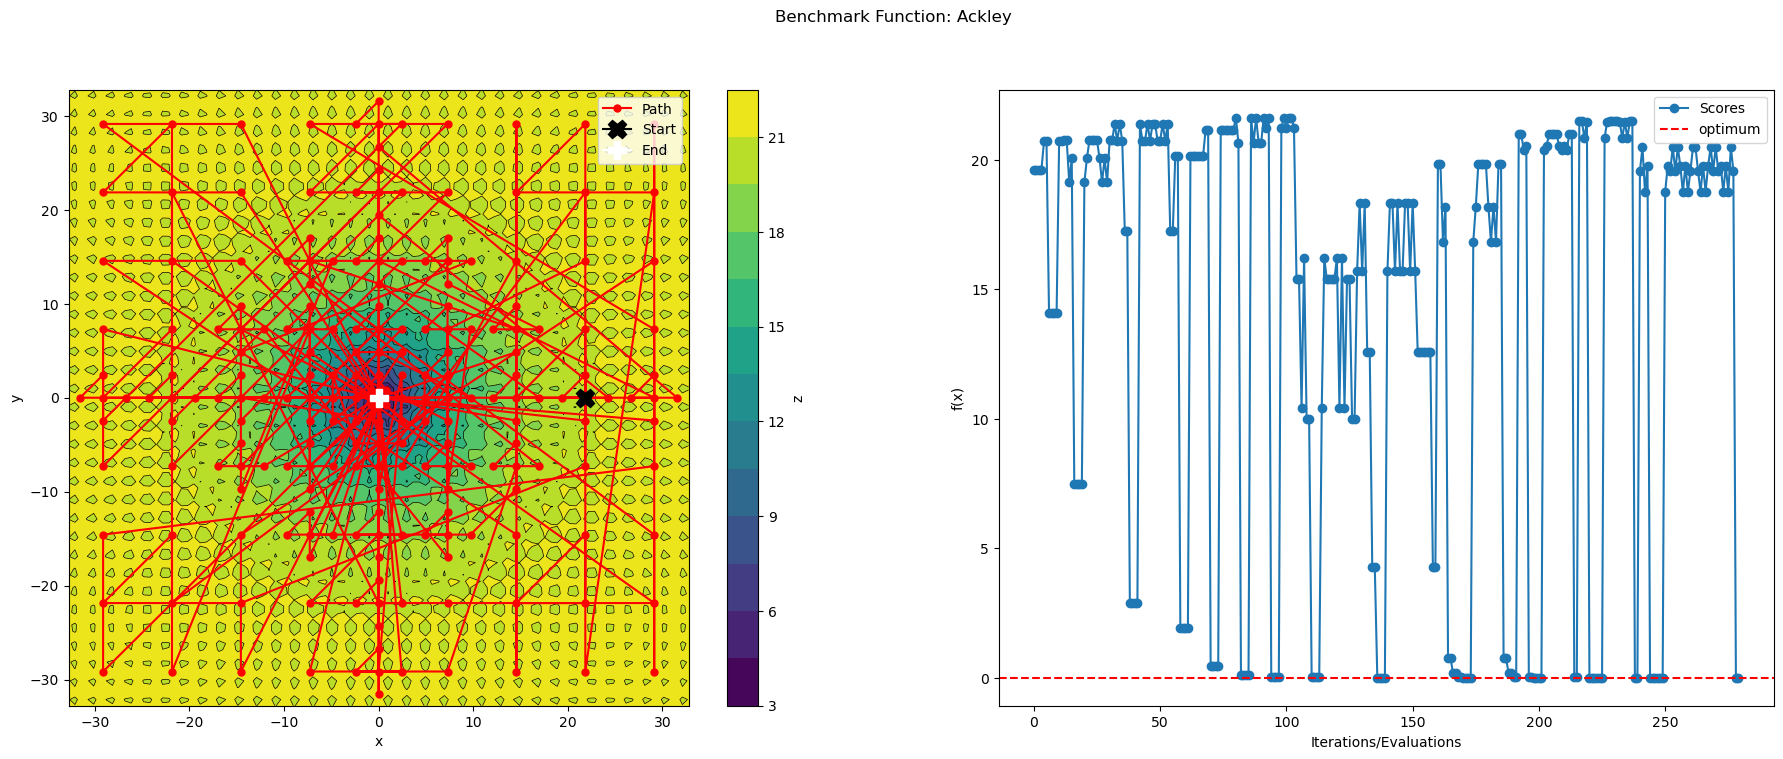
\includegraphics[width=\textwidth]{lab2/imgs/di_ackley_eps_01.png}
        \caption{$\epsilon =0.1$}
    \end{subfigure}
    \begin{subfigure}{0.5\textwidth}
        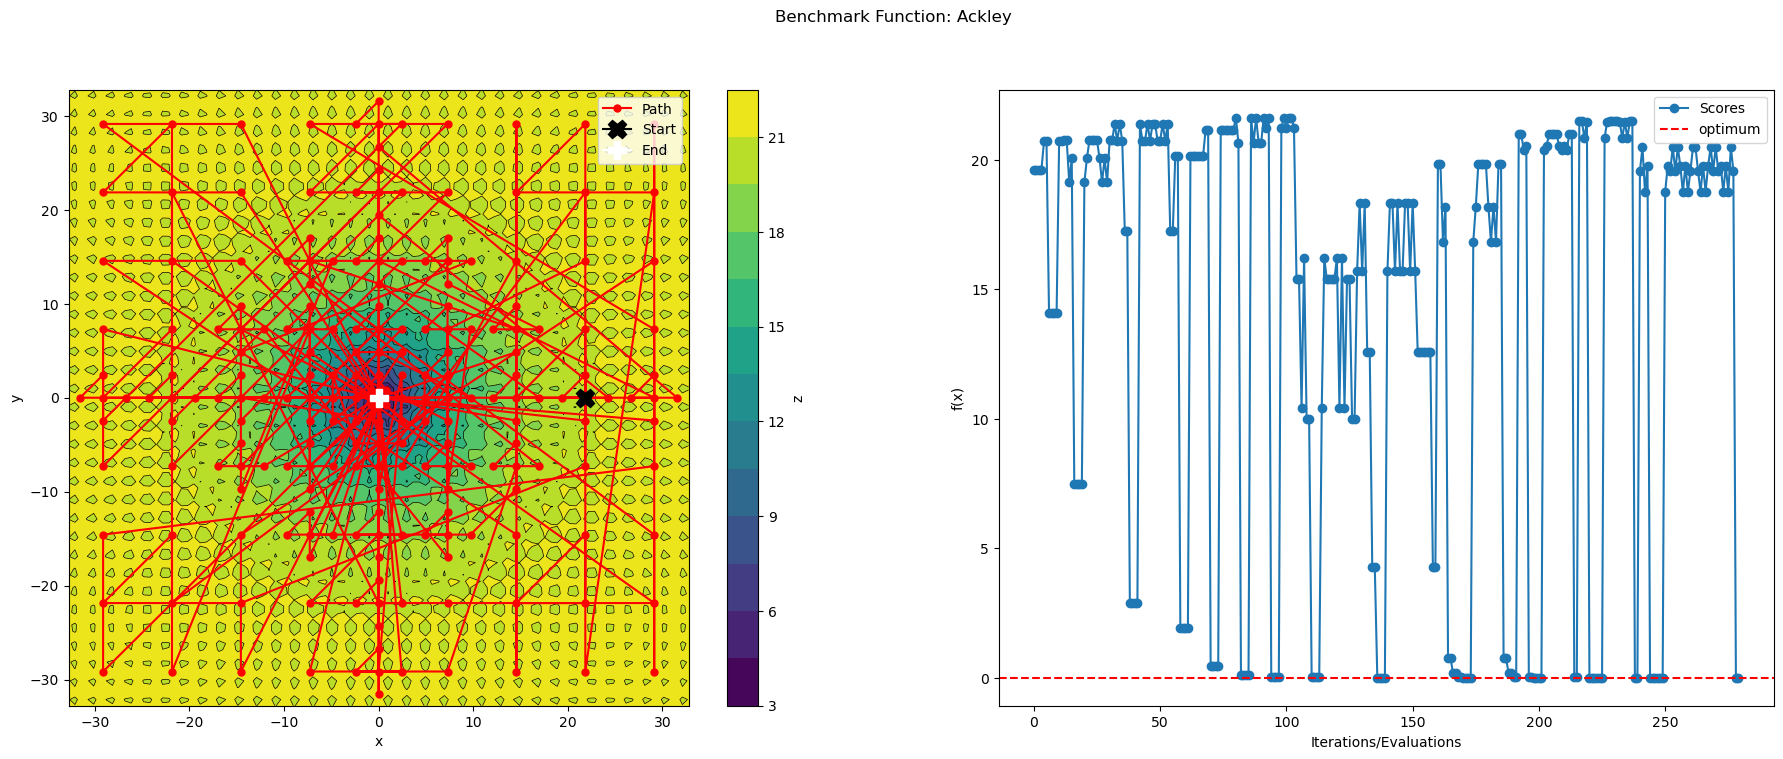
\includegraphics[width=\textwidth]{lab2/imgs/di_ackley_eps_001.png}
        \caption{$\epsilon =0.001$}
    \end{subfigure}
    \caption{DIRECT on Ackley's function with different tolerances}
    \label{fig:ackley-tolerance}
\end{figure}

As we would expect, a larger number of iterations leads to a better approximation of the global minimum, in some more extreme cases even changing the basin of attraction of the global minimum. This is the case for the De Jong's function \ref{fig:dejong-iterations} where the minimum found is significantly different for different numbers of evaluations.
\begin{figure}[H]
    \begin{subfigure}{0.5\textwidth}
        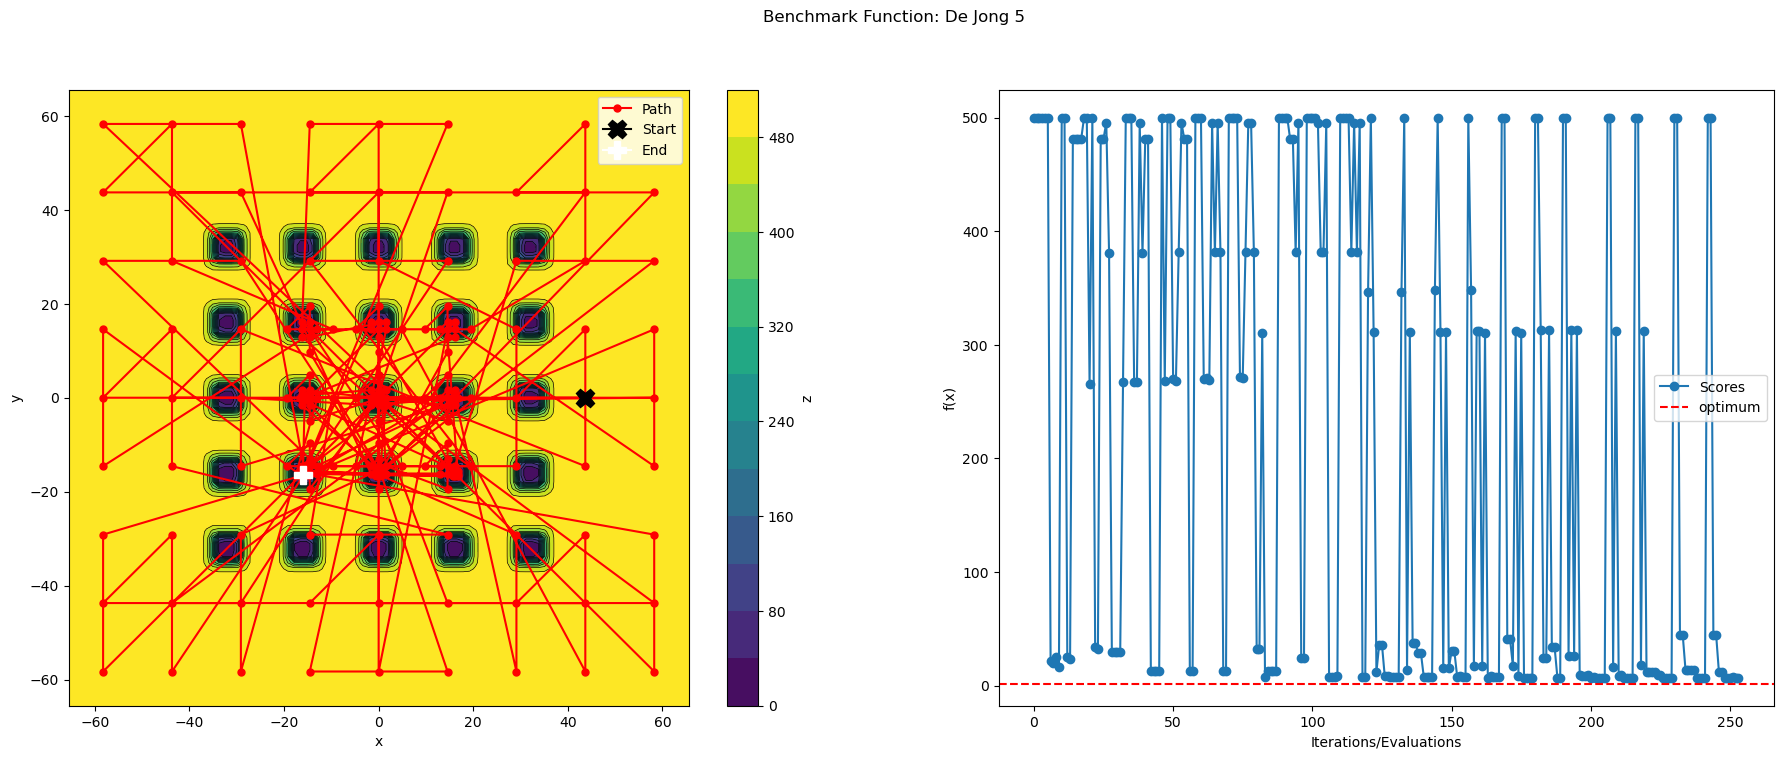
\includegraphics[width=\textwidth]{lab2/imgs/di_i100_e250.png}
        \caption{100 iterations and 250 evaluations}
    \end{subfigure}
    \begin{subfigure}{0.5\textwidth}
        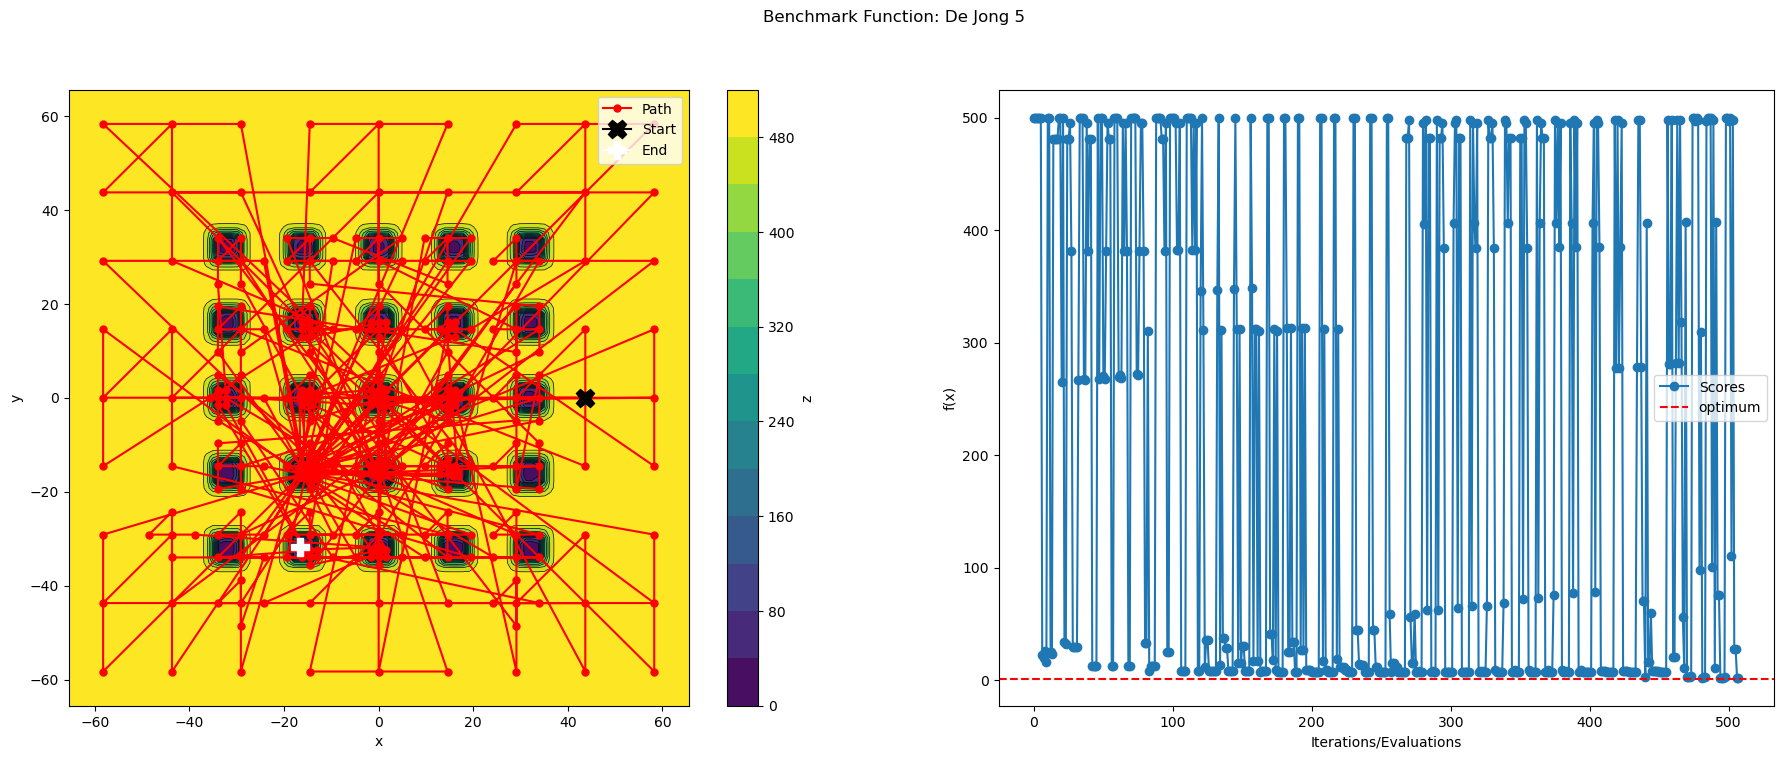
\includegraphics[width=\textwidth]{lab2/imgs/di_i100_e500.png}
        \caption{100 iterations and 500 evaluations}
    \end{subfigure}\\
    \begin{subfigure}{\textwidth}
        \centering
        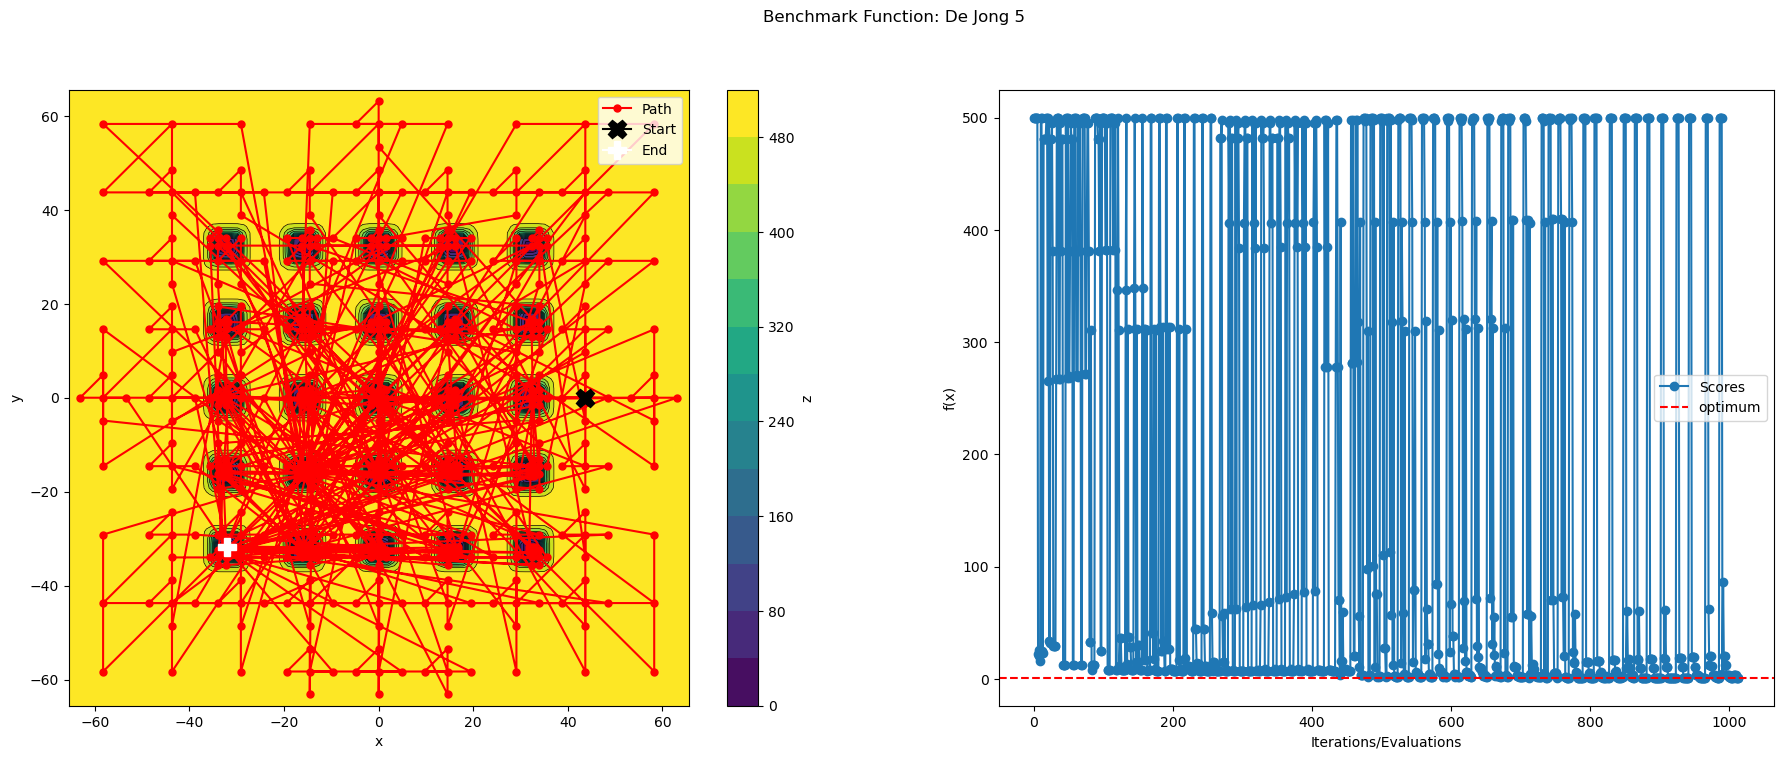
\includegraphics[width=0.5\textwidth]{lab2/imgs/di_i100_e1000.png}
        \caption{100 iterations and 1000 evaluations}
    \end{subfigure}
    \caption{DIRECT on De Jong's function with different number of evaluations}
    \label{fig:dejong-iterations}
\end{figure}

Another interesting thing to note is the behaviour of the algorithm with a large number of local minima and how we can see how DIRECT evaluations are much more spread out compared to other functions. This can be seen really well in the Griewank function \ref{fig:griewank}.
\begin{figure}[H]
    \centering
    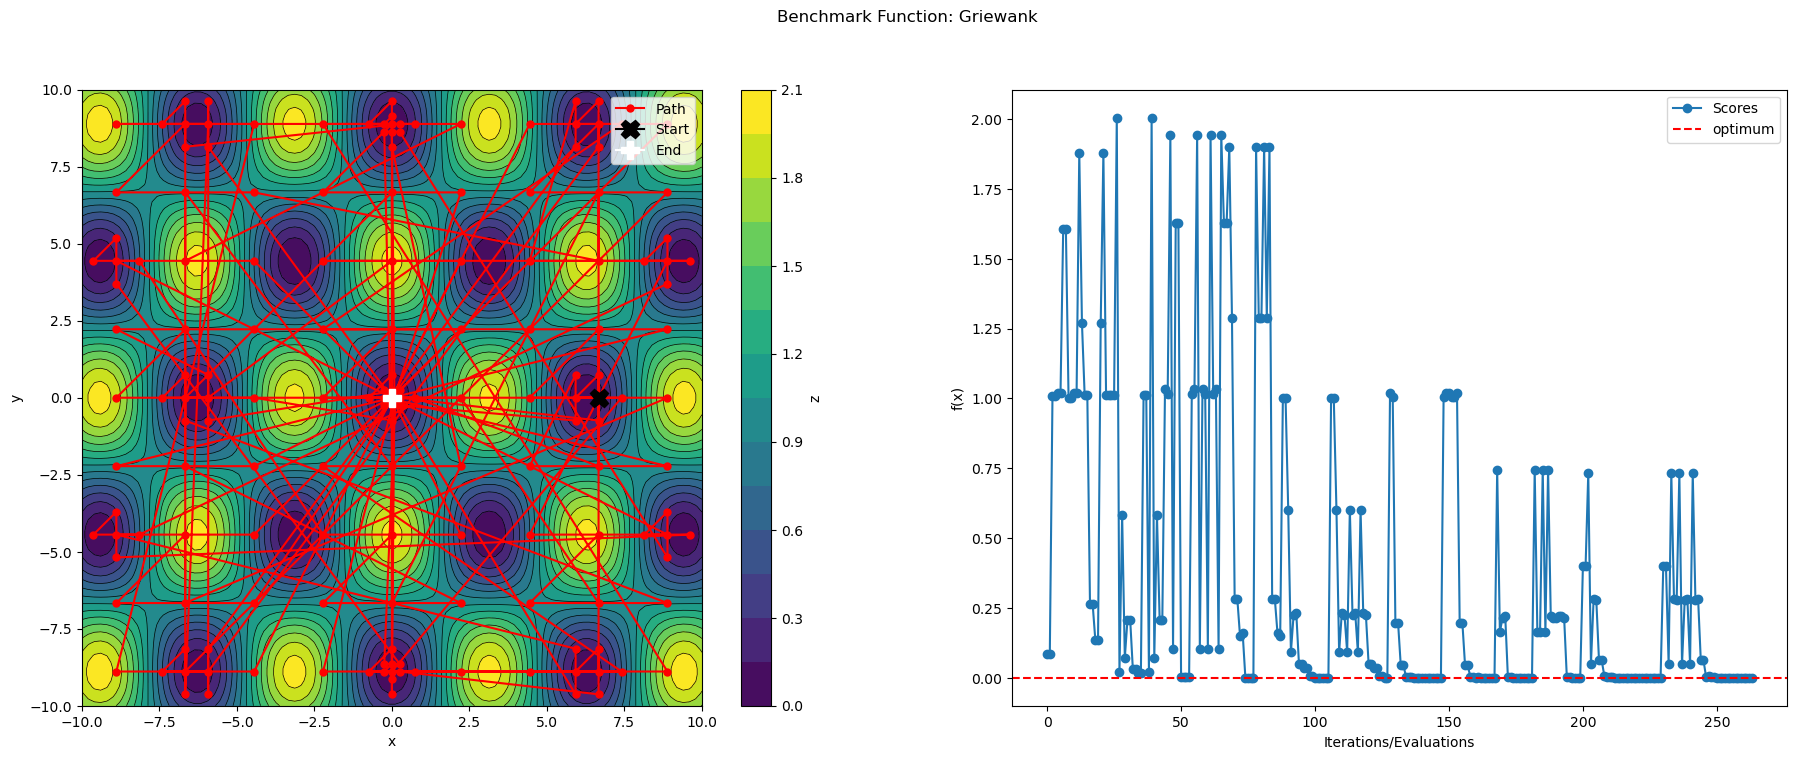
\includegraphics[width=0.8\textwidth]{lab2/imgs/griewank.png}
    \caption{DIRECT on Griewank's function}
    \label{fig:griewank}
\end{figure}

\subsection{Basin Hopping}
Basing Hopping is a form of Iterated Local Search with a different starting point each time. It loops through the following steps:
\begin{enumerate}
    \item \textit{Hopping}: perturbation of the current solution ("jump" to new parts of the search space)
    \item \textit{Local Search}: perturbed solution is optimized using a local search method
    \item \textit{Acceptance} the new solution is accepted or rejected based on an acceptance criterion. This criterion can be defined in different ways; here is defined based on the Metropolis criterion.
\end{enumerate}
It's particularly important to set the temperature and the stepsize parameters correctly as specified in the scipy documentation. In particular:
\begin{enumerate}
    \item \textit{Temperature}: usually set to be comparable with with the separation of the objective function value of local minima.
    \item \textit{Stepsize}: should be set to be comparable to the Distance in the coordinates between local minima.
\end{enumerate}

For example, we can see how the algorithm behaves with the Dejong5 function \ref{fig:bh-dejong} with different temperatures (10 and 0.1) and that the temperature has a significant impact on the evaluations: The higher temperature leads to a more spread out evaluation of the function because the algorithm is more likely to accept worse solutions and leave the local basin of attraction.
\begin{figure}[H]
    \begin{subfigure}{0.5\textwidth}
        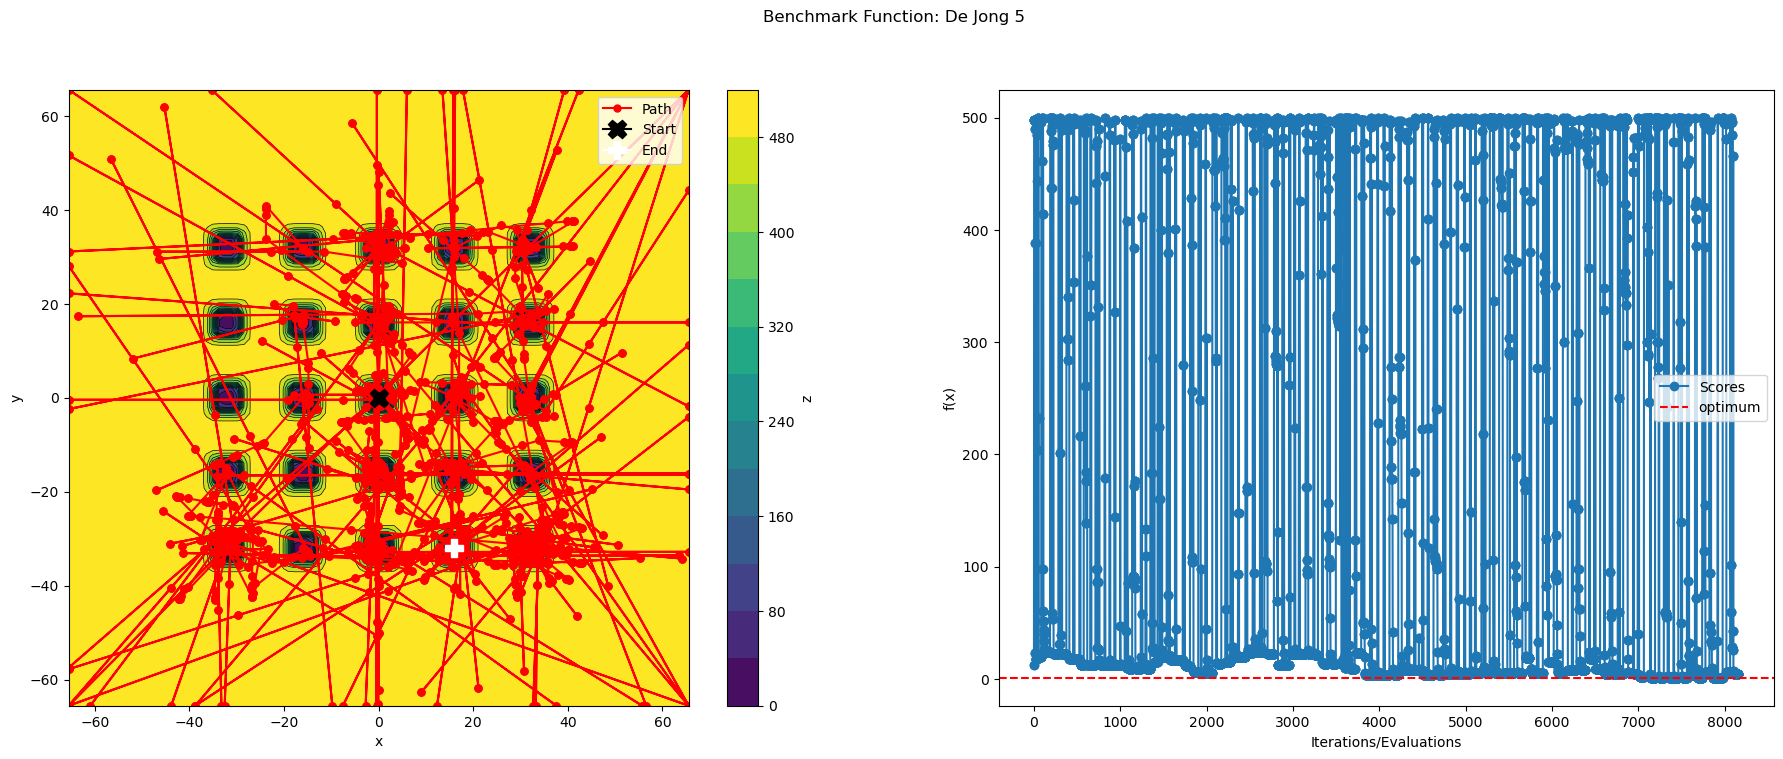
\includegraphics[width=\textwidth]{lab2/imgs/bh_dejong_10.png}
        \caption{Temperature = 10}
    \end{subfigure}
    \begin{subfigure}{0.5\textwidth}
        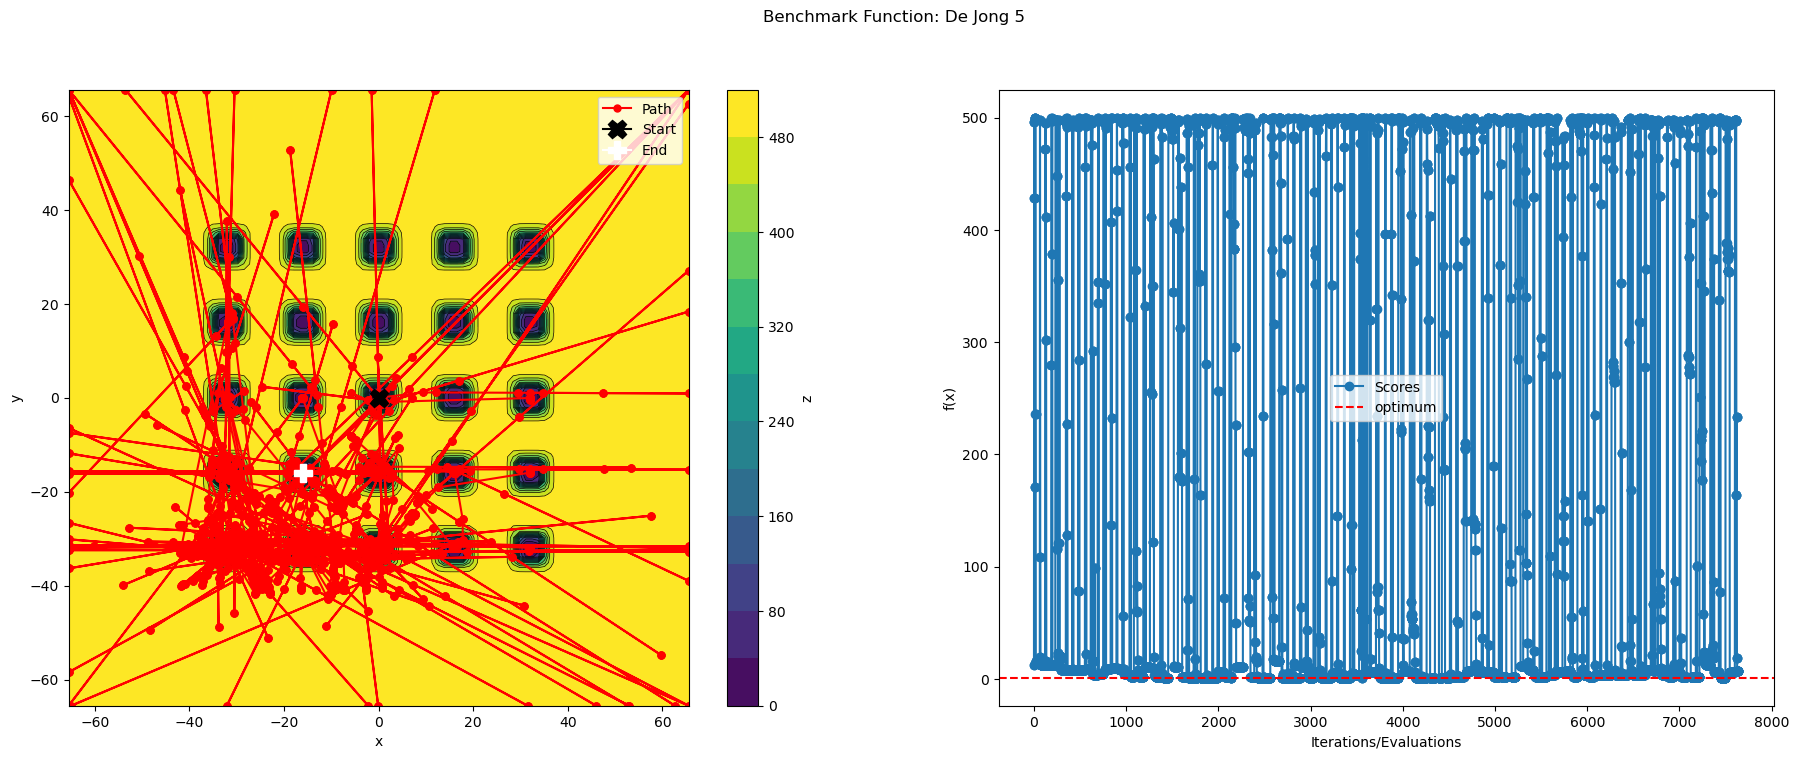
\includegraphics[width=\textwidth]{lab2/imgs/bh_dejong_01.png}
        \caption{Temperature = 0.1}
    \end{subfigure}
    \caption{Basin Hopping on De Jong's function with different temperatures and stepsize 20}
    \label{fig:bh-dejong}
\end{figure}
The importance of the stepsize can be seen by comparing the previous results with the ones obtained with a stepsize of 1 (Figure \ref{fig:bh-dejong-stepsize}) where we can clearly see that the algorithm isn't able to leave the local basin of attraction.
\begin{figure}[H]
    \centering
    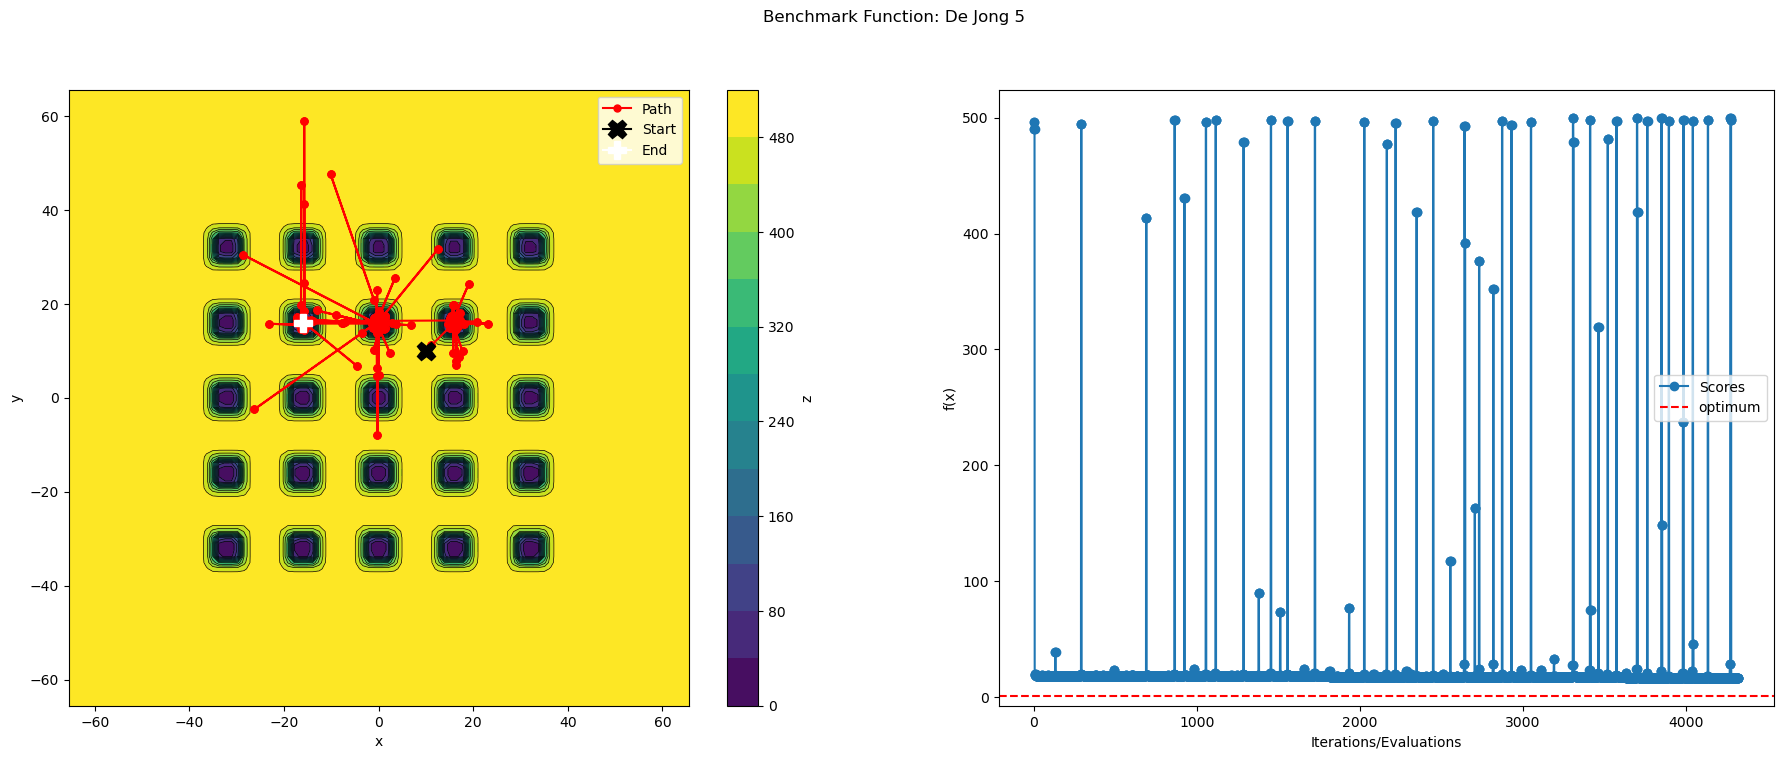
\includegraphics[width=0.8\textwidth]{lab2/imgs/bh_dejong_step_1.png}
    \caption{Basin Hopping on De Jong's function with stepsize = 1}
    \label{fig:bh-dejong-stepsize}
\end{figure}

It's also interesting to note that, even if the global minimum is found, this isn't necessarily the last evaluation of the function. This makes sense because the only stopping condition is the number of iterations, so the algorithm will continue to evaluate the function even after finding the global minimum. 

If we have a unimodal function, such as the Rosenbrock function \ref*{fig:bh-rosenbrock}, the algorithm is able to immediately find the global minimum via the local search step.
\begin{figure}[H]
    \centering
    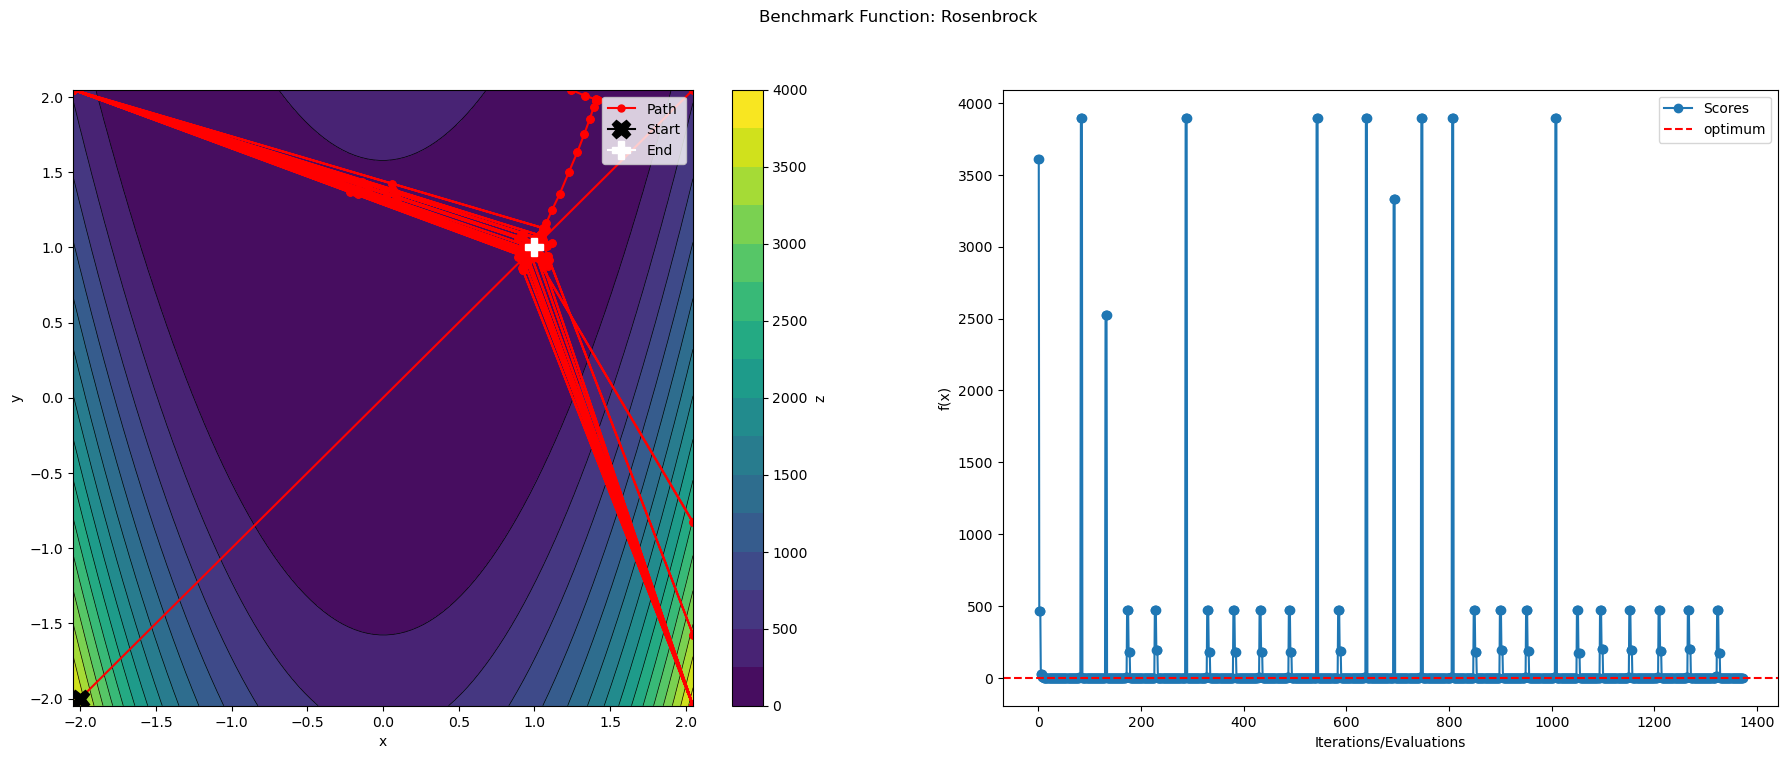
\includegraphics[width=0.8\textwidth]{lab2/imgs/bh_rosenbrock.png}
    \caption{Basin Hopping on Rosenbrock's function}
    \label{fig:bh-rosenbrock}
\end{figure}

\noindent
\textbf{Note}: the code was slightly modified to add bounds to the local search algorithm (L-BFGS-B) to avoid the algorithm from going out of bounds.

